\documentclass[]{usiinfbachelorproject}
\usepackage{subfigure, wrapfig, url, array, caption,xcolor,amsmath,algorithm, tikz}
\usepackage{footnotebackref}
\usepackage[english]{babel}
\usepackage[noend]{algpseudocode}

\newcommand\tab[1][1cm]{\hspace*{#1}}
\captionsetup{labelfont={bf}}

%%% For algorithms %%%
\makeatletter
\def\BState{\State\hskip-\ALG@thistlm}
\makeatother
%%%%%%%%%%%%%

\newcommand\transp[1]{{#1}^{\top}}

\author{Vanessa Braglia}

\title{The swiss scientific social network}
\versiondate{\today}

% DA SCOMMENTARE
\begin{committee}
\advisor[Universit\`{a} della Svizzera Italiana, Switzerland]{Prof.}{Olaf}{Schenk}
\assistant[Universit\`a della Svizzera Italiana, Switzerland]{}{Fabio}{Verbosio}
\end{committee}

\abstract {
In this project I implemented some algorithms to analyze the swiss scientific social network.
To construct the graph representing the relations (the edges) between authors (the nodes) I crawled some conferences' online programs and I have extracted all the necessary information. I used PageRank and graph partitioning to study the relationships between authors: I found the members that collaborate more with each other and the relationship between different institutions. The results provide an interesting picture of the different research scenarios in Switzerland and how they interact with each other internally to an establishment but also between different institutions. 
}


\begin{document}
% DA SCOMMENTARE
\maketitle
\newpage
\tableofcontents
\newpage

%%%%%%%%%%%%%%%%%%%%%%%%%
\section{Introduction} \label{sec:intro} 
%%%%%%%%%%%%%%%%%%%%%%%%%

A social network consists of a set of objects connected to each other by social relations. The best way to model social networks is using graphs: the objects (entities) are represented as nodes and the connections as edges between two different nodes (see Figure \ref{fig:socialnetwork}). The most common example we can take is the World Wide Web (WWW) where we have web pages as nodes connected by hyperlinks, the edges.

\begin{figure}[ht]
	\centering
	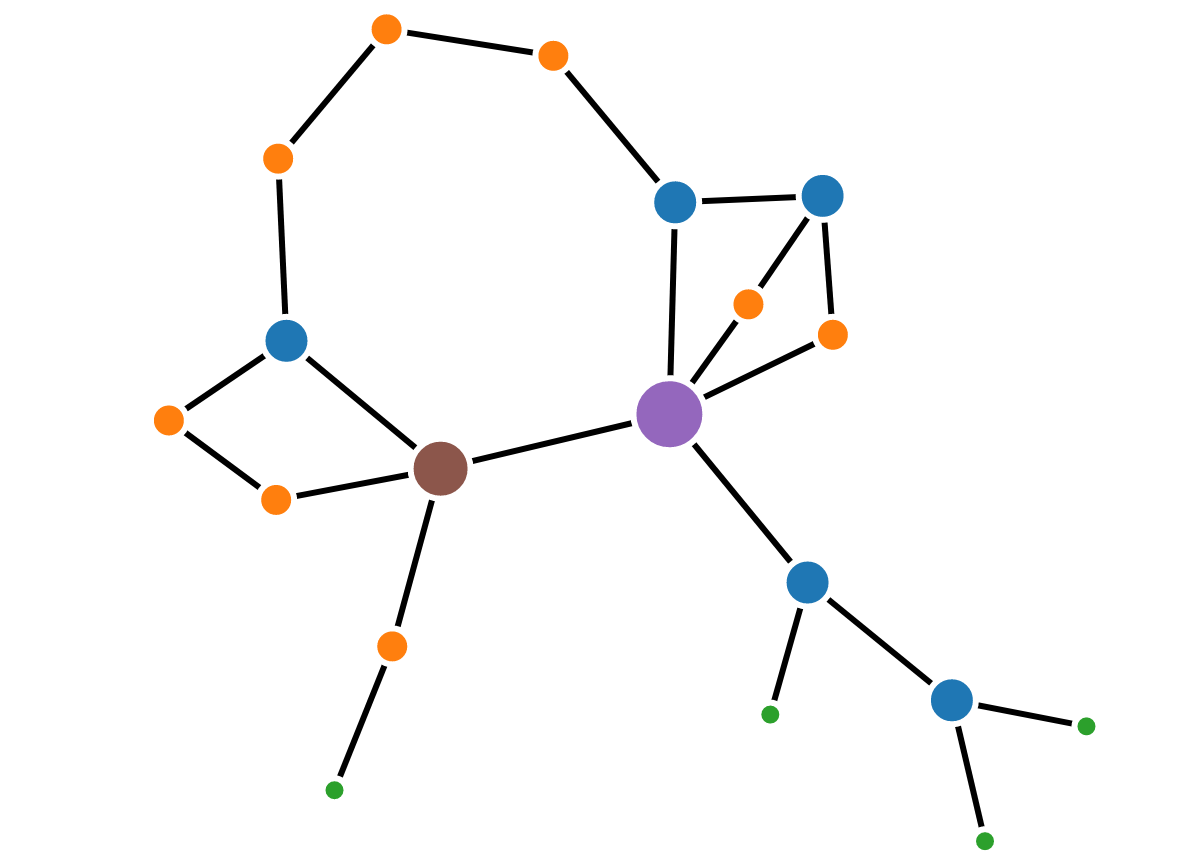
\includegraphics[height=4cm]{img/graph2.png}
	\caption{Example of social network graph}
	\label{fig:socialnetwork}
\end{figure}

The goal of this project is to create a social network of computational science authors belonging to Swiss institutions and corporations, and then analyze the relative graph, represented by an adjacency matrix. I want to find the relations between authors of the same or different institutions and belonging to the same or to different research scenarios: how they interact with each other and if they are strictly related to the institution or cooperate throughout Switzerland. The result will provide also a ranking of the authors and the institutions to see which are the most influential in the computational science research.

The first step is retrieving all the necessary information for the construction of the social network, i.e., names of the authors and relationships between each other. I crawled the 2015, 2016 and 2017 PASC Conferences and different SIAM conferences of several years, selecting the topics relevant to us (e.g. Optimization, Parallel Computing,...). The PASC conferences are interdisciplinary and bring together researchers across the areas of computational science, high-performance computing, and various domain sciences.

The second step is the information analysis to find out relations between institutions and between members belonging to the same or different institutes. With PageRank algorithm we obtain a ranking of all the conference participants; it is an algorithm used by Google Search to rank websites in their search engine results, but it can be applied to any social network. 

In this project I use the algorithm to measure the importance of the institution members considering the number and quality of their collaborations and to find out the relevant universities for computational science researches. 

I use graph partitioning techniques to invert the process, trying to obtain the institutions from members collaborations: it is reasonable to assume that members of the same institution collaborate more between each other than with other institutions' representatives. With this assumption the algorithm will cut the relations between members of different universities, keeping the representatives of each institution in the same group.

I also analyze the institutions connectivity matrices and their structure: looking at the cliques present in the matrices, we can for example detect the different research areas of the institutions and the connection between them. Cliques are dense sub matrices which represent a group of authors that are closely connected with each other. 

The results will provide an interesting picture of the different research scenarios in Switzerland and how they interact with each other.






%%%%%%%%%%%%%%%%%%%%%%%%%
\section{Information Retrieval} \label{sec:inforetrieval} 
%%%%%%%%%%%%%%%%%%%%%%%%%
Information retrieval is the process of extracting, starting from an information need, the relevant information from a collection of resources. In this project, the necessary information are the names of the institutions members and the collaborations between them. 
First, I try to use Mendeley API but it allows only to take 100 results per query and there is no control on the type of information to be retrieved. Additionally, it does not return all the information needed, i.e., not all authors have a specified institution and only few papers were available.

After this first unproductive attempt to use Mendeley API, I decide to  extract the information from some online conferences programs: the idea is that if two authors presented some work together at a conference, then they are connected in my social network.

I crawl the conference programs and I construct a parser to extract the information from the HTML pages and to organize the data.

\subsection{Crawling}

A web crawler is an Internet bot that browses the World Wide Web, typically for the purpose of web indexing of search engines. In this project the goal is not indexing web pages but save the information contained in the HTML to parse them and construct the social network.

The web pages that I decide to crawl are the online programs of 2015, 2016 and 2017 PASC conferences and of SIAM conferences with arguments concerning computational science i.e., Optimization, Parallel Computing, Computational Science \& Engineering, Imaging Science, Uncertainty Quantification, Linear Algebra in Signals, Systems \& Control, Data Mining and Analysis of Partial Differential Equations.

I use Apache Nutch~\cite{nutch}, a highly extensible and scalable open source web crawler, allowing the user to crawl a lot of web pages with few command lines.
It starts with a list of URLs to visit, called the seeds; I create this list including all the links to the computational science conferences web pages previously mentioned.

As the crawler visits the URLs, it identifies all the hyperlinks in the page and adds them to the list of URLs to visit; in my case I crawl only the pages in the starting seed ignoring all the internal links. The crawler copies and saves the information as it goes and stores in a repository each page as a distinct file.

Thanks to Apache Nutch I manage to create a text file with the HTML of all the saved conference pages. After this file is created, the next step is studying the structure of the page and how to extract the information needed, i.e., where we can find the information in the page, if it is included in some particular HTML tag, and how to interpret it. In order to do so, I designed a parser responsible for these tasks.

\subsection{Parsing}
A parser is a program that receives data as input and breaks it up into smaller elements that can then be used for different purposes. In this project, the parser reads the text file created after the crawling and extracts from it the information about Swiss institutions and their members. The data obtained is used to create the social network ready to be analyzed.

In this project I personally write a parser, using Python programming language, to extract the information from the conferences HTML pages. The parser goes through the structure of the page and extracts only the useful information. Clearly, different page structures require different parser, then I write two of them because the SIAM conferences and the PASC have different structures.

The parser extracts only the lines of the pages which contain the names of the authors, their institutions and nationality; the institutions members that present a work together at a conference appear in group in the page so I keep them together to later extract the relations. Thanks to the nation expressed in the program I can differentiate the Swiss authors from the rest of the the world. 

Once that the desired lines are collected, I take the groups one after the other, and I extract name, institution, nation and coauthors for each member. With all this information I manage to construct a social network and its corresponding adjacency matrix.

In case a single author belongs to two distinct institutions I decide to include two different entries because I'm interest in institutions collaborations: so the same author can have some coauthors with one university and completely different coauthors with the other one. We can see an example in Figure \ref{fig:twoUni} where professor Olaf Schenk is affiliated to two different universities (Universit\`{a} della Svizzera Italiana and Univerisity of Basel) and collaborates with Matthias Bolhoefer from both institutions but he works with Fabio Verbosio only from USI and with Marcus Grote only from the University of Basel.
\begin{figure}
\begin{center}
\tikzset{every picture/.style={line width=0.75pt}}      

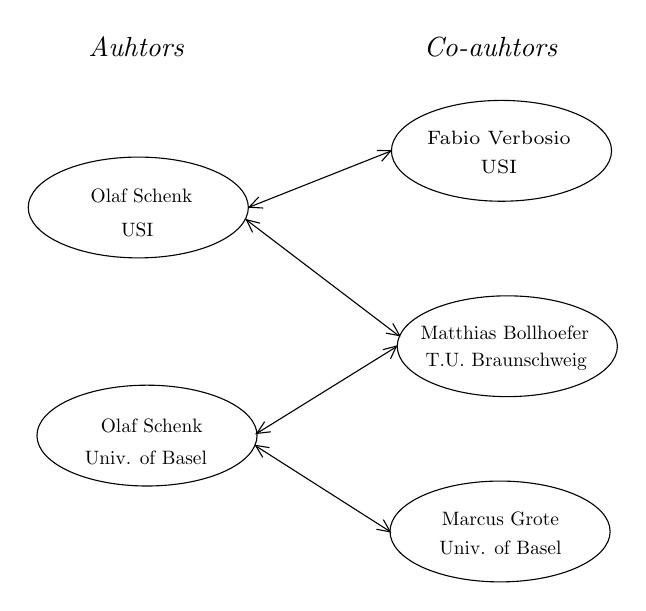
\begin{tikzpicture}[x=0.75pt,y=0.75pt,yscale=-0.7,xscale=0.7]

\draw    (186.75,311) -- (279,369.8) ;


\draw    (181.5,146.8) -- (280,107.8) ;


\draw    (359.75, 242.3) circle [x radius= 75.75, y radius= 34.7]  ;
\draw    (179.75,155) -- (284.25,234.5) ;


\draw    (186.5,302.8) -- (284,242.3) ;


\draw    (354.75, 369.8) circle [x radius= 75.75, y radius= 34.7]  ;
\draw    (355.75, 107.8) circle [x radius= 75.75, y radius= 34.7]  ;
\draw    (105.75, 146.8) circle [x radius= 75.75, y radius= 34.7]  ;
\draw    (111.75, 303.8) circle [x radius= 75.75, y radius= 34.7]  ;
\draw [rotate around= { 336.14: (275.61, 109.5)
    }]  (271.23,105.42) -- (279.99,109.5) -- (271.23,113.58) ;
\draw [rotate around= { 158.13: (186.11, 145)
    }]  (181.73,140.92) -- (190.49,145) -- (181.73,149.08) ;
\draw [rotate around= { 219.28: (183.61, 158)
    }]  (179.23,153.92) -- (187.99,158) -- (179.23,162.08) ;
\draw [rotate around= { 35.54: (282.11, 232.5)
    }]  (277.73,228.42) -- (286.49,232.5) -- (277.73,236.58) ;
\draw [rotate around= { 214.12: (190.11, 313)
    }]  (185.73,308.92) -- (194.49,313) -- (185.73,317.08) ;
\draw [rotate around= { 148.5: (191.11, 300)
    }]  (186.73,295.92) -- (195.49,300) -- (186.73,304.08) ;
\draw [rotate around= { 35.54: (275.61, 367.5)
    }]  (271.23,363.42) -- (279.99,367.5) -- (271.23,371.58) ;
\draw [rotate around= { 320.3: (280.11, 245)
    }]  (275.73,240.92) -- (284.49,245) -- (275.73,249.08) ;

\draw (108,139) node [scale=0.7] [align=left] {Olaf Schenk};
\draw (105,162) node [scale=0.7] [align=left] {USI};
\draw (355,361) node [scale=0.7] [align=left] {Marcus Grote};
\draw (355,381) node [scale=0.7] [align=left] {Univ. of Basel};
\draw (354,99) node  [align=left] {{\scriptsize Fabio Verbosio}};
\draw (354,119) node  [align=left] {{\scriptsize USI}};
\draw (358,233) node [scale=0.7] [align=left] {Matthias Bollhoefer};
\draw (359,253) node [scale=0.7] [align=left] {T.U. Braunschweig};
\draw (115,297) node [scale=0.7] [align=left] {Olaf Schenk};
\draw (111,319) node [scale=0.7] [align=left] {Univ. of Basel};
\draw (105,36) node  [align=left] {\textit{Auhtors}};
\draw (349,36) node  [align=left] {\textit{Co-auhtors}};

\end{tikzpicture}
\caption{Example of author with two different universities and different coauthors} \label{fig:twoUni}
\end{center}
\end{figure}

One of the big issues of my dataset was that the institutions were labeled differently. For example, the Swiss university \textit{ETH Z\"{u}rich} can also be named \textit{ETHZ} or \textit{Swiss Federal Institute of Technology Zurich}.  Moreover there can be some organizations of the university such as the \textit{ETHZ Computational Laboratory} or the \textit{Institute of Fluid Dynamics}. All these names have to be represented by the same institution label. 

To solve this problem I construct an hash map putting the label to use as key and a list with all names represented by that label as value. For example the one for ETH Z\"{u}rich will have: 
\begin{itemize}
\item label:  ``ETHZ''
\item value:  [``ETH Z\"{u}rich'',``Swiss Federal Institute of Technology Zurich'', ``ETHZ Computational Laboratory'', ``Institute of Fluid Dynamics'']
\end{itemize}

For each university I scan this map and reassign the corresponding name.

I make two different databases, one for Switzerland and one for the whole world. The first one contains only Swiss authors and their collaborations with members of the same nation, while in the second there are also authors other nations and their collaborations are extended to all over the world. For each author I save the name, the university, the nation, a list of his coauthors and I assign to each of them a unique index. 

From this data set I easily create the adjacency matrix and thanks to the indexes I can switch between the matrix and the database; from the graph I can read the index and go in the database to see to which author it corresponds.





%%%%%%%%%%%%%%%%%%%%%%%%%
\section{The PageRank Algorithm} \label{sec:pagerank} 
%%%%%%%%%%%%%%%%%%%%%%%%%
PageRank is an algorithm used by Google Search to rank websites in their search engine results. It was developed by  Larry Page and  Sergey Brin (the Google founders) in 1996 as part of their research project at Stanford University~\cite{pagerank}.

PageRank is used, together with other algorithms, to measure the importance of web pages and sort them by popularity in the results; it can be used on any graph to compute the importance of each node by its PageRank value. Larry Page and  Sergey Brin algorithm works by counting the number and quality of links to a page, to compute a value which represents its importance: more popular a page is, more likely it receives links from other websites and even more likely from important websites.

\begin{figure}[ht]
	\centering
	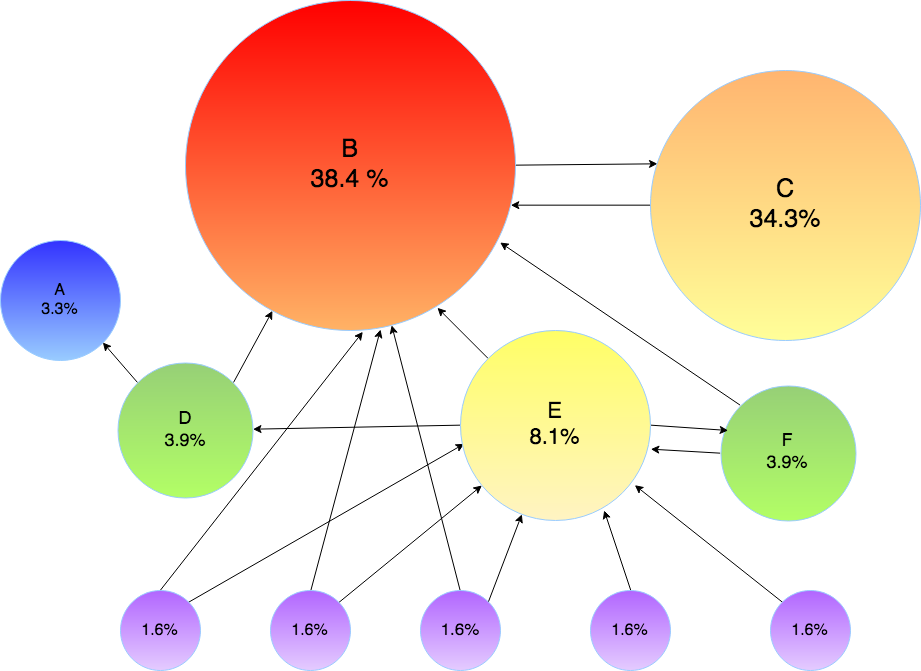
\includegraphics[height=6cm]{img/page_rank_example.png}
	\caption{PageRank example}
	\label{fig:prexample}
\end{figure}

As we can see in Figure \ref{fig:prexample}, node C has higher PageRank than A even if it has the same number of inner links; this is because the only inner link of C is from the most important node of the graph, B, so it is considered to be more important than the inner link on node A.

While surfing websites, going from one page to another, I want to avoid problems with pages without outer links so I introduce two different methods to choose the next page. The surfer can:
\begin{itemize}
\item randomly choose an outgoing link from the page, or
\item choose a random page from the network.
\end{itemize}
We assume that the surfer follows the first option with probability $p$ (typically $p=0.85$) and the second with probability $1-p$. This theoretical random walk is known as a Markov chain or Markov process.

The probability that an infinite random surfer visits a specific website is called its PageRank; a page will have high rank if other pages with high rank link to it.


\subsection{How to compute PageRank values}
To apply PageRank, from a graph of $n$ nodes we construct a $n$-by-$n$ connectivity matrix G such that
\begin{equation*}
g_{ij}=1 \text{\;\;\; if and only if nodes $i$ and $j$ are connected.} 
\end{equation*}
The number of non-zeros in $G$ is the total number of connections in the graph.

The scalar $r_i$ represents the number of inner-links of page $i$, while column $c_i$ the number of outer-links. So we can define:
\begin{itemize}
\item In-degree of page $i$: \tab $\:\:\:\:r_i = \sum\limits_{j=1}^{n} g_{ij}$
\item Out-degree of page $i$: \tab $c_i = \sum\limits_{j=1}^{n} g_{ji}$
\end{itemize}
Since the collaboration is a symmetric relation, my graph is undirected, hence the number of inner-links is equal to the number of outer-links. 

Let $p$ be the probability that the surfer follows a link and $1-p$ the probability that it chooses a random page, then $\delta = \frac{1-p}{n}$ is the probability that a particular random page is chosen.

We construct a transition probability matrix A, where all the elements are positive and smaller than one, and the sum of each column is equal to one.
The last property comes from the fact that column $j$ represents the probabilities to go from page j to all other pages. So, we set
\begin{equation}\notag
a_{ij} = 
\begin{cases}
\frac{pg_{ij}}{c_{j}} + \delta  & \text{if } c_{j} \neq 0\\
\frac{1}{n} & \text{if } c_{j} = 0
\end{cases}.
\end{equation}
In other words, if page $j$ has no outer links, it means that column $j$ of $A$ present a uniform probability $\frac{1}{n}$ in all its elements. Since matrix A is a transition matrix of a Markov chain~\cite[Chapter 7]{markov}, all its eigenvalues are real, between 0 and 1, and 1 is an eigenvalue itself
$$0 \leq \lambda_1 \leq \lambda_2 \leq \dots \leq \lambda_n = 1 \text{.}$$
We can now compute PageRank values by solving the problem 

\begin{equation}\notag
A\:x = x \text{.}
\end{equation}

This is a particular eigenvalue problem (for more details see~\cite[Chapter 8]{eigs}) of the form $Ax=\lambda x$, where, in our specific case, $\lambda = 1$. We compute the eigenvector relative to the greatest eigenvalue, which is 1 as just mentioned.

The transition matrix $A$ can be written as
$$A = pGD+ez^{T}, $$
where $D$ is a diagonal matrix with the reciprocals of the out-degrees, i.e.,
\begin{equation}\notag
d_{jj} = 
\begin{cases}
\frac{1}{n} & \text{if } c_{j} \neq 0\\
0 & \text{if } c_{j} = 0
\end{cases} \,,
\end{equation}
$z$ is the vector formed by
\begin{equation}\notag
z_{j} = 
\begin{cases}
\delta & \text{if } c_{j} \neq 0\\
\frac{1}{n} & \text{if } c_{j} = 0
\end{cases} \,,
\end{equation}
and $e$ is the vector of length $n$ with all ones. For more details about this, see~\cite[Chapter 7]{molerPR} (https://ch.mathworks.com/moler/chapters.html).

We can write the linear system
$$(I-A)x=0$$
as
$$(I - pGD)x = \gamma e$$
where $\gamma = \transp{z}x$.
To conclude, since the value of the scalar $\gamma$ depends on the unknown $x$, we impose the condition $\gamma = 1$, then solve
\begin{equation}\notag
(I - pGD)x = e
\end{equation}
and then rescale the solution so that $\sum\limits_{i=1}^{n} x_i = 1$.

\begin{algorithm}
\caption{ (PageRank)}\label{pagerank}
\begin{algorithmic}[1]
\Procedure{PageRank}{}
\State $\textit{U} \gets \text{list of }\textit{authors}$
\State $\textit{G} \gets \text{adjacency matrix}$
\State $p \gets \text{dumping factor}$
\State $\textit{G} \gets \textit{G} - \text{diag(}\textit{G}\text{)} \: \: \: \text{(remove self collaborations)}$
\State $\textit{c} \gets \text{sum(}\textit{G}\text{,1)} \:\:\: \textit{r} \gets \text{sum(}\textit{G}\text{,2)} \:\:\: \text{(Compute out-degree and in-degree of each node)}$
\State $\textit{D} \gets \text{Diagonal matrix with reciprocals of out-degrees}$
\State Solve $(I - pGD)x = e$
\State $x \gets x / sum(x) \: \:\: \text{(normalize the result x)}$
\State $x \gets \text{sort x in descending order}$\\
\Return x
\EndProcedure
\end{algorithmic}
\end{algorithm}






%%%%%%%%%%%%%%%%%%%%%%%%%
\section{The Graph Partitioning Algorithm} \label{sec:graphpart} 
%%%%%%%%%%%%%%%%%%%%%%%%%
Graph partitioning consists in dividing a graph $G=(V,E)$\footnote{A graph G with vertexes V and edges E.}  cutting the smaller number of edges and obtaining sub-graphs with specific properties. K-way partitioning of a graph G of n nodes, consists in a division of its nodes in k disjoint subset, all with size nearly $\frac{n}{k}$ (see Figure \ref{fig:kpartitioning}). The idea is just to apply the spectral partitioning $\frac{k}{2}$ times recursively to each of the partitions obtained. The method is presented in Algorithm~\ref{kpartitioning}.

\begin{figure}[ht]
	\centering
	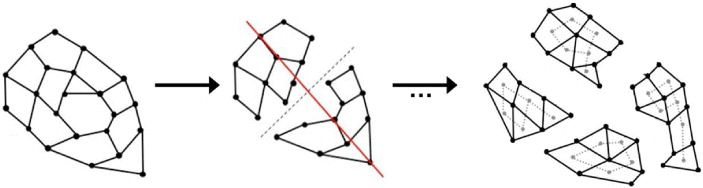
\includegraphics[height=3cm]{img/k_way_partitioning.jpg}
	\caption{Example of k-way graph partitioning}
	\label{fig:kpartitioning}
\end{figure}

\begin{algorithm}
\caption{ (k-way Partitioning)}\label{kpartitioning}
\begin{algorithmic}[1]
\Procedure{k-way Partitioning}{}
\State $\textit{G} \gets \text{(V,E)}$
\State $k \gets \text{number of desired partitions}$
\State $\text{Apply spectral partitioning on G and find }G_1 \text{ and } G_2$
\BState \emph{loop}:
\If {$\frac{k}{2} > 1$}
\State $\text{Recursive partition on }G_1 \text{ with } \frac{k}{2}$
\State $\text{Recursive partition on }G_2 \text{ with } \frac{k}{2}$
\State $k \gets \frac{k}{2}$
\EndIf
\State \textbf{goto} \emph{loop}\\
\Return $G_1 = (V_1,E_1) \text{ ... } G_K = (V_K,E_K)$
\EndProcedure
\end{algorithmic}
\end{algorithm}

A partitioning algorithm is said to be efficient if it divides a given graph into smaller components with about the same size, cutting as few edges as possible. 
A valid and fast method is the coordinate bisection, which simply chooses a partitioning plane perpendicular to one of the coordinate axes but spectral algorithm is more efficient. It finds a partition based on the eigenvalues and eigenvectors of the Laplacian matrix of the graph and doesn't need the nodal coordinates.

%As we can see in Figure \ref{fig:partitioning} sometimes coordinate and spectral partitioning behave similarly but usually the second one is more effective even if it cuts more edges.
%\begin{figure}[ht]
%	\centering
%	\subfigure[]{
%		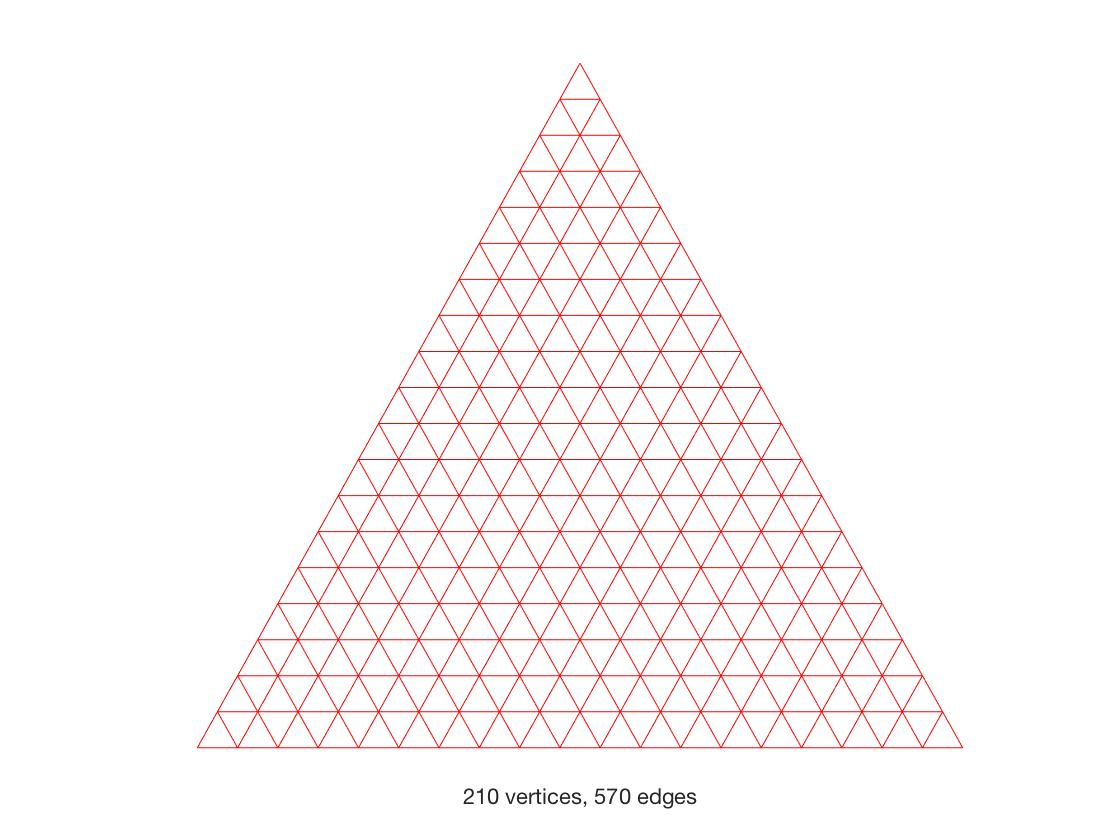
\includegraphics[height=4cm]{img/g4.jpg}
%		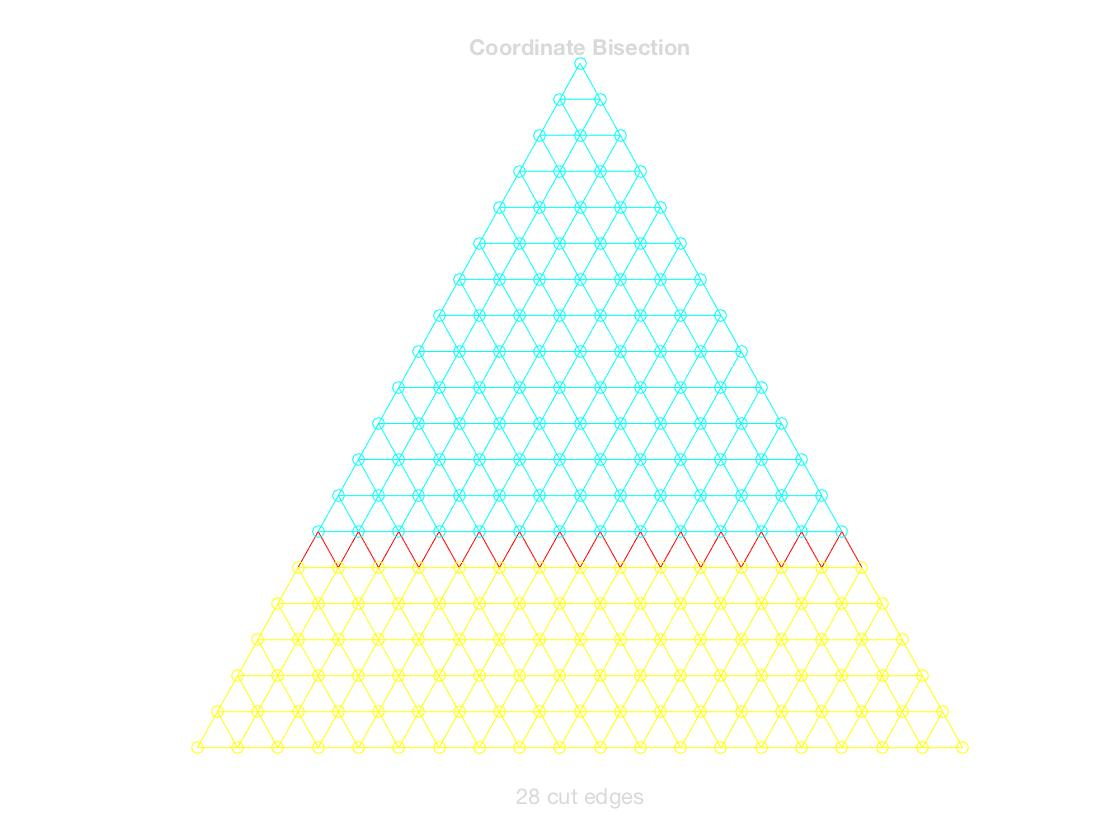
\includegraphics[height=4cm]{img/g5.jpg}
%		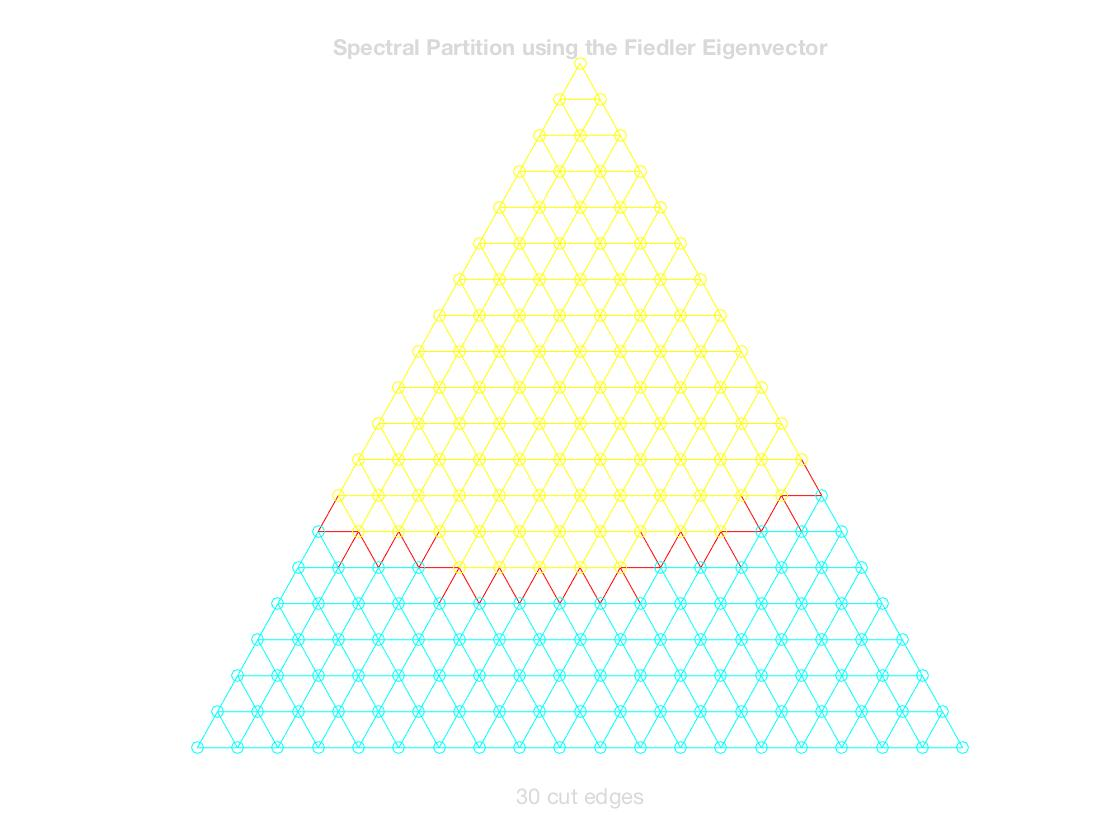
\includegraphics[height=4cm]{img/g6.jpg}
%		\label{fig:corandsp}
%	}
%	\subfigure[]{
%		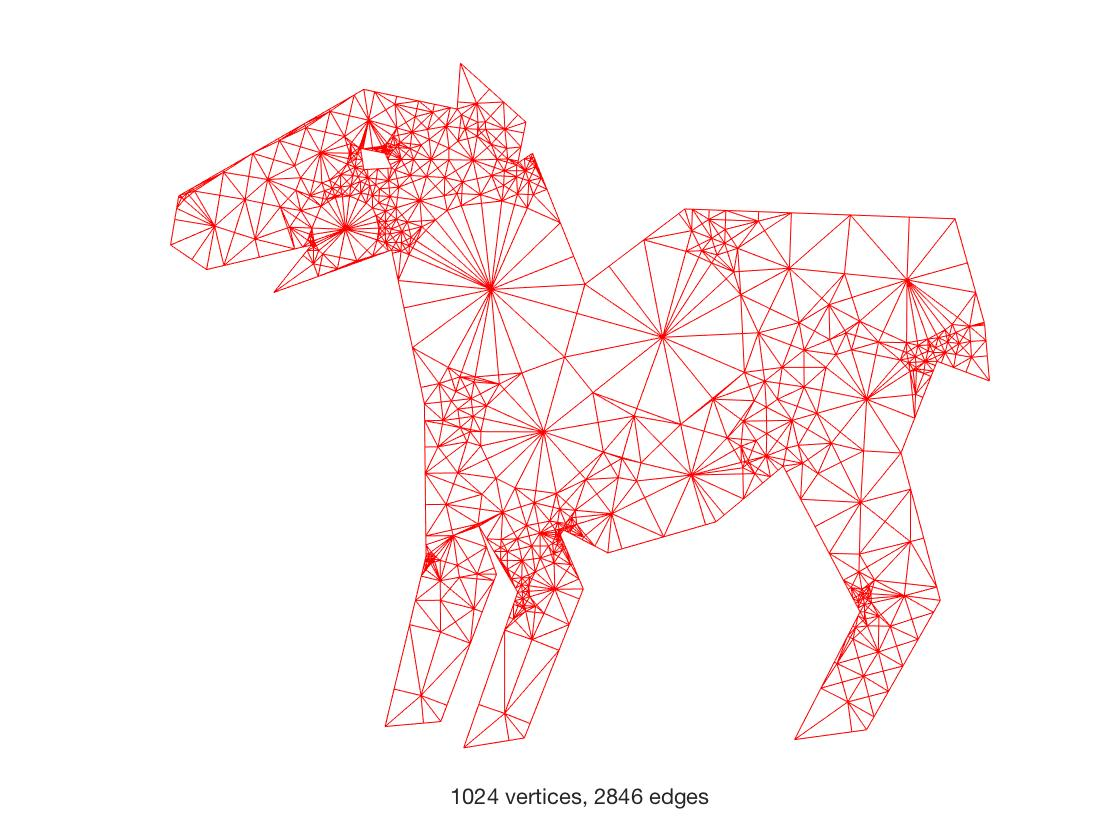
\includegraphics[height=4cm]{img/g10.jpg}
%		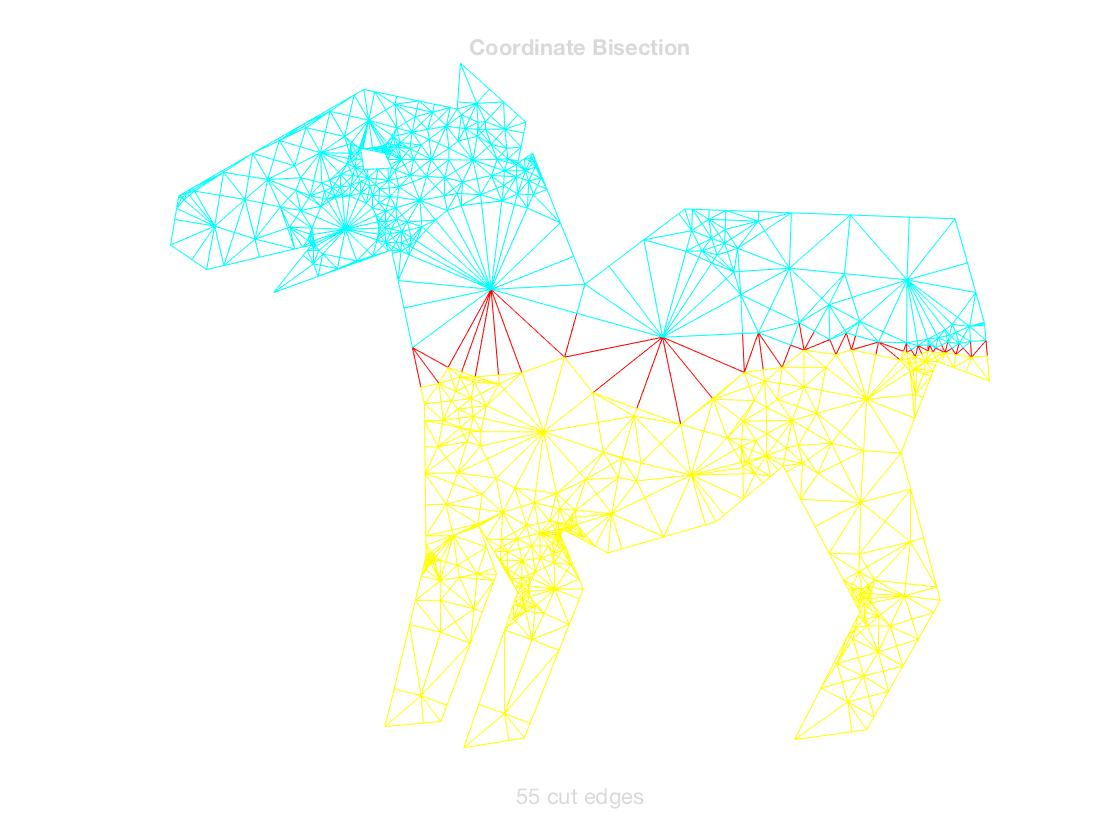
\includegraphics[height=4cm]{img/g11.jpg}
%		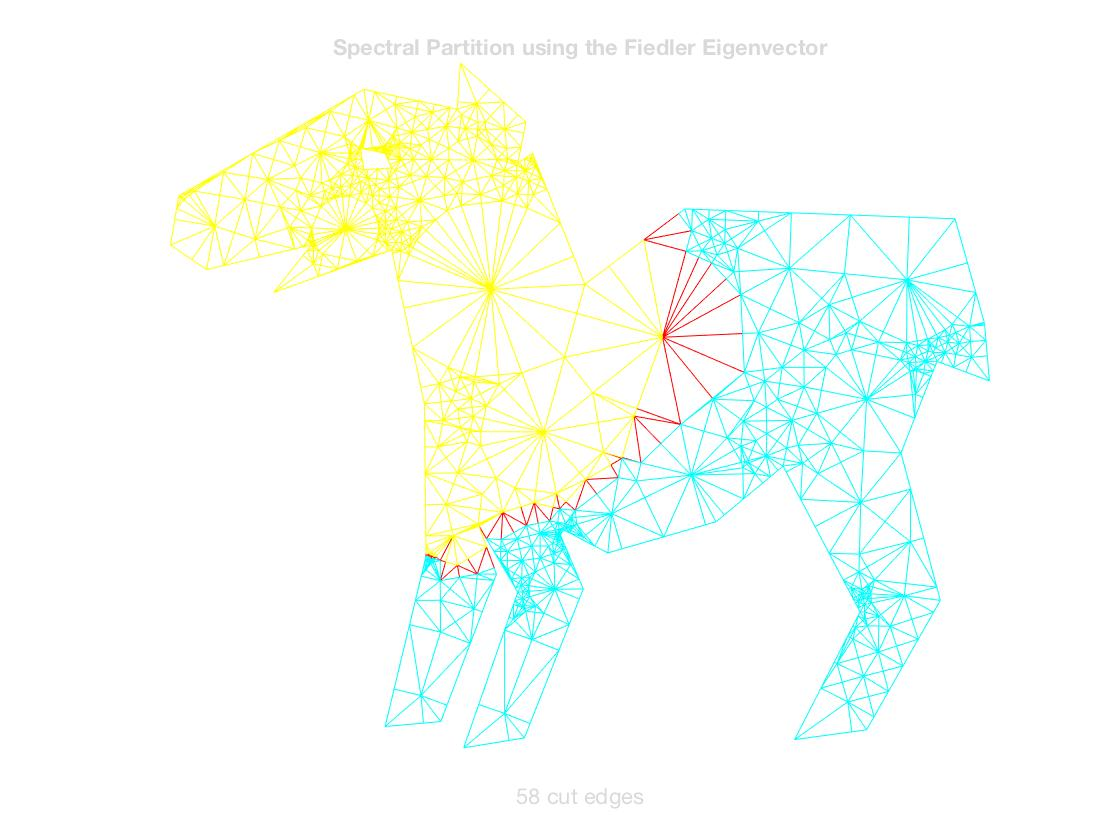
\includegraphics[height=4cm]{img/g12.jpg}
%		\label{fig:cororsp}
%	}
%	\caption{In both \subref{fig:corandsp} and \subref{fig:cororsp} we have the graph at the left, the coordinate bisection in the middle and the spectral partition on the right}
%	\label{fig:partitioning}
%\end{figure}

\subsection{How to apply spectral graph partitioning}
To apply graph partitioning we need the adjacency matrix $A$ of the graph, which is symmetric since the graph is considered to be undirected, and the Laplacian matrix $L$ constructed such that: 
\begin{equation}\notag
L_{ij} = 
\begin{cases}
d_i \tab \:\:\: if \:\: i=j \\
-1 \tab if \:\: i \neq j \:\: and \: \: (i,j) \in E \\
0 \tab \:\:\:\: \text{otherwise}
\end{cases}
\end{equation}
where $d_i$ is the vertex degree of node $i \in V$.
The relation between A and L is
\begin{equation}\notag
L = D - A
\end{equation}
where D is the diagonal matrix having the $d_i$'s on the diagonal. Since L is symmetric and positive semidefinite by construction, all its eigenvalues are real and nonnegative. The first eigenvalue is always zero and, in the general case, the multiplicity of the the first eigenvalue corresponds to the number of connected components of the graph.

The eigenvalues of L are ordered as follows:
\begin{equation}\notag
0 = \lambda_1 = \ldots = \lambda_m < \lambda_{m+1} \le \ldots \lambda_n
\end{equation}

The eigenvector corresponding to the first eigenvalue $\lambda_1$ is the vector of all ones and it does not provide information about the graph structure; the second lowest eigenvector, instead, called ``Fiedler eigenvector'', is used by spectral partitioning to return the smaller sub-graphs. Dividing the nodes of graph G according to the median $s$ of the Fiedler vector $v = (v_1,v_2,...,v_n)$ gives two partitions $V_1$ and $V_2$ such that
\begin{equation}\notag
\begin{cases}
v_i \in V_1 \text{\;\; if \;\;} v_i \leq s \\
v_i \in V_2 \text{\;\; if \;\;} v_i > s
\end{cases} .
\end{equation}
Such a partition is called the Fiedler cut and leads to two parts of G with nearly equal number of vertexes, minimizing the number of cut edges. 

Fiedler theorem said that if the graph G is connected, L the Laplacian matrix, $N_+$ and $N_-$ a partitioning such that
\begin{equation}\notag
x(i) = +1 \tab \text{if } v_i \text{in } N_+ 
\end{equation}
\begin{equation}\notag
x(i) = -1 \tab \text{if } v_i \text{in } N_-
\end{equation}

Then the number of edges cut is:
\begin{equation}\notag
\#\text{edge\_cut} = \frac{1}{4}x^T L x
\end{equation}

This problem of minimizing the number of cut edges is NP-hard and can be written as a constrained minimization problem:
\begin{equation}\notag
\min\limits_z f(z)=\frac{1}{4} z^T L z \tab \text{subject to} \tab 
\begin{cases}
z^T z = n \tab \text{z is a real vector}\\
z^T e = 0 \tab \text{with } e=[1,1,...,1]^T
\end{cases}
\end{equation}








%%%%%%%%%%%%%%%%%%%%%%%%%
\section{Numerical analysis}
%%%%%%%%%%%%%%%%%%%%%%%%%
After retrieving all the necessary information and organizing the data in adjacency matrices, I applied the PageRank algorithm, obtaining the following results.
Since the Swiss author names obtained are only 422, I decide to extend the research to the institutions from all over the word, reaching 16425 names. So the analysis is done in parallel for both Swiss collaborations and authors from all over the world.

I first construct the adjacency matrices of the authors and their corresponding institutions; for the organizations I also build a weighted matrix which keeps stored the number of collaborations between them. I consider that each author collaborates with himself so the diagonal of the matrix will contain ones.
We can see in Figure \ref{fig:authorsAdj} the authors matrices, while in Figure \ref{fig:univAdj} the one of the Swiss institutions.

\begin{figure}[tb]
	\centering
	\subfigure[]{
		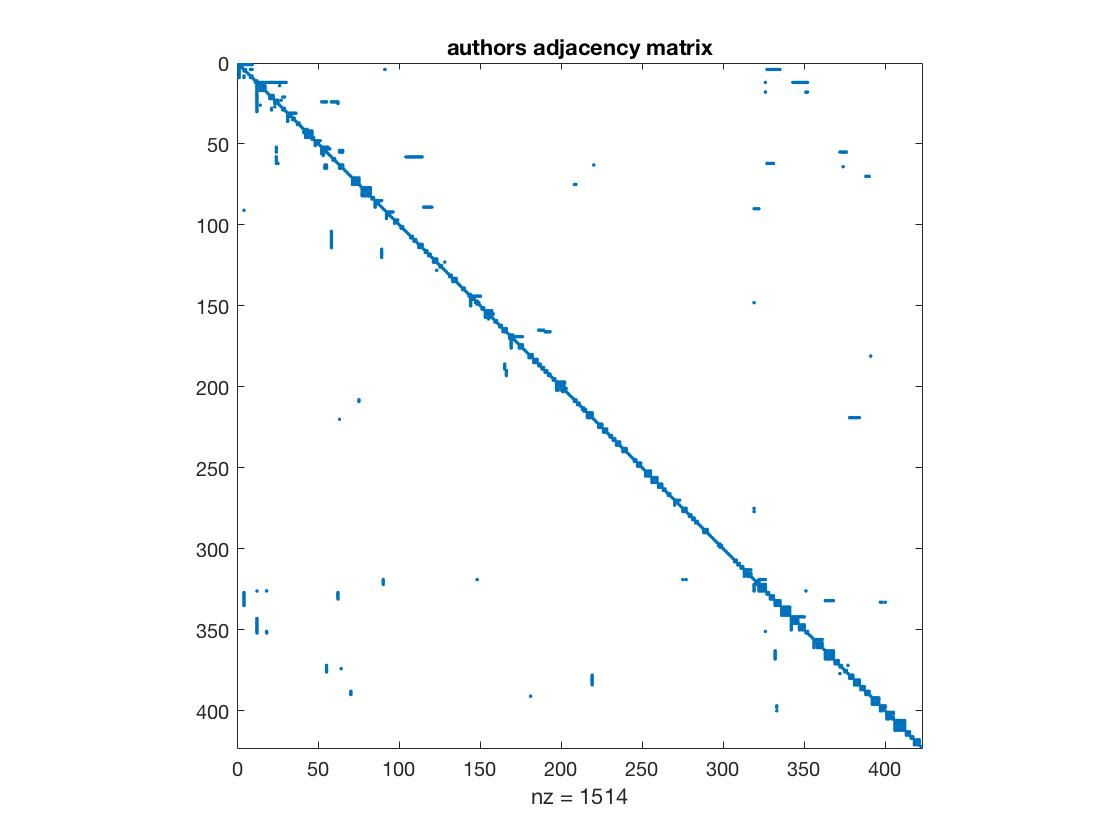
\includegraphics[height=4.5cm]{img/Analysis/authors_adj.jpg}
		\label{fig:AdjS}
	}
	\subfigure[]{
		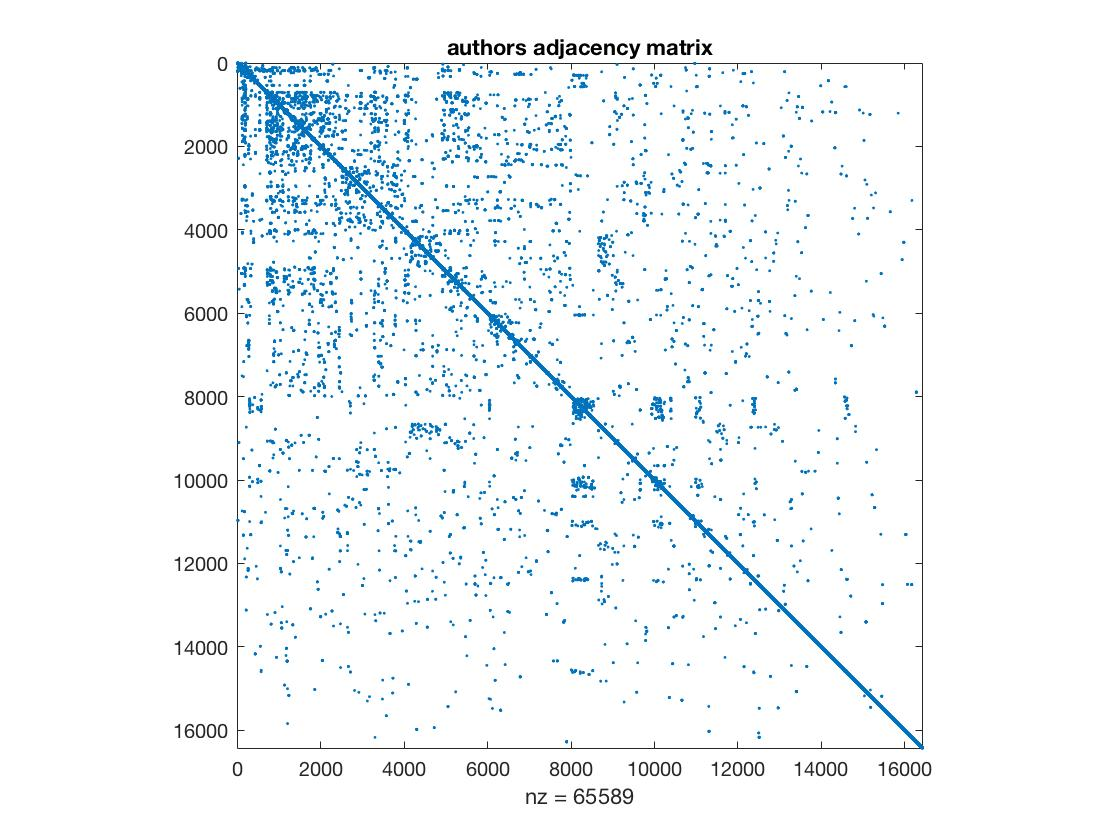
\includegraphics[height=4.5cm]{img/Analysis_world/author_adj.jpg}
		\label{fig:AdjW}
	}
	\caption{\subref{fig:AdjS} is the Swiss authors' adjacency matrix and \subref{fig:AdjW} is the one of the world authors}
	\label{fig:authorsAdj}
\end{figure}

\begin{figure}[tb]
	\centering
	\subfigure[]{
		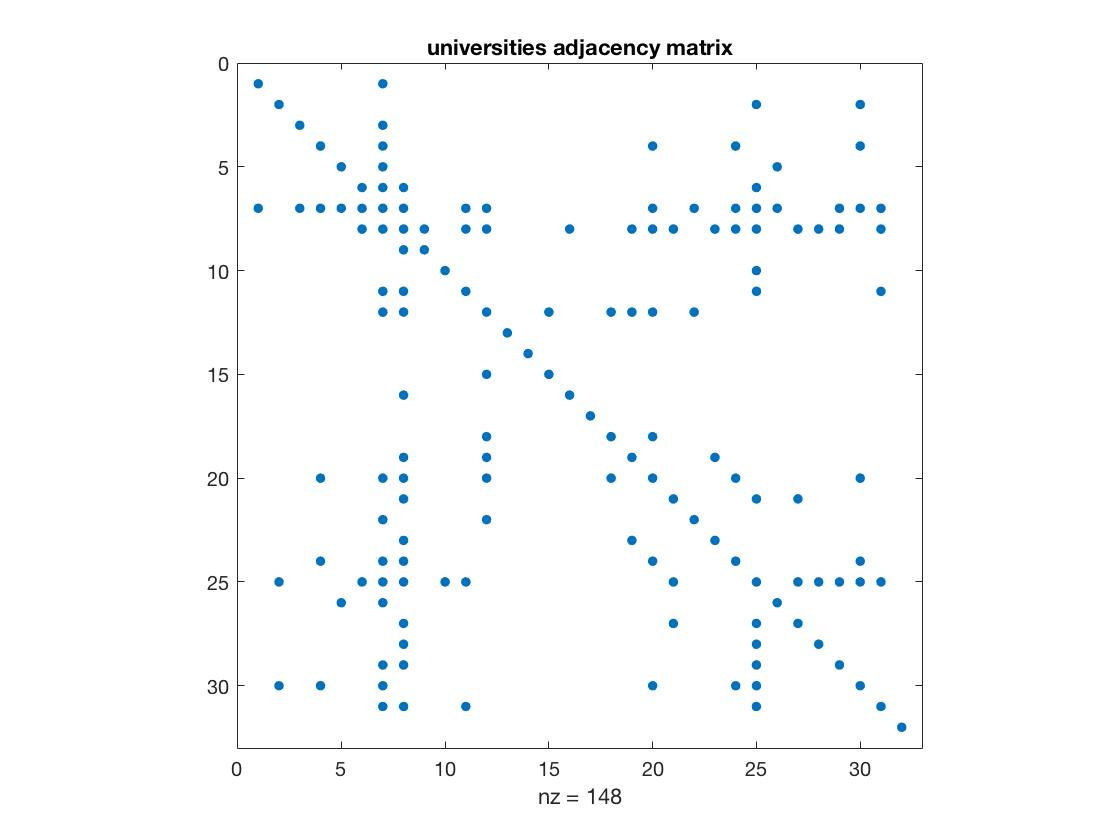
\includegraphics[height=4.5cm]{img/Analysis/univ_adj.jpg}
		\label{fig:uniAdj}
	}
	\subfigure[]{
		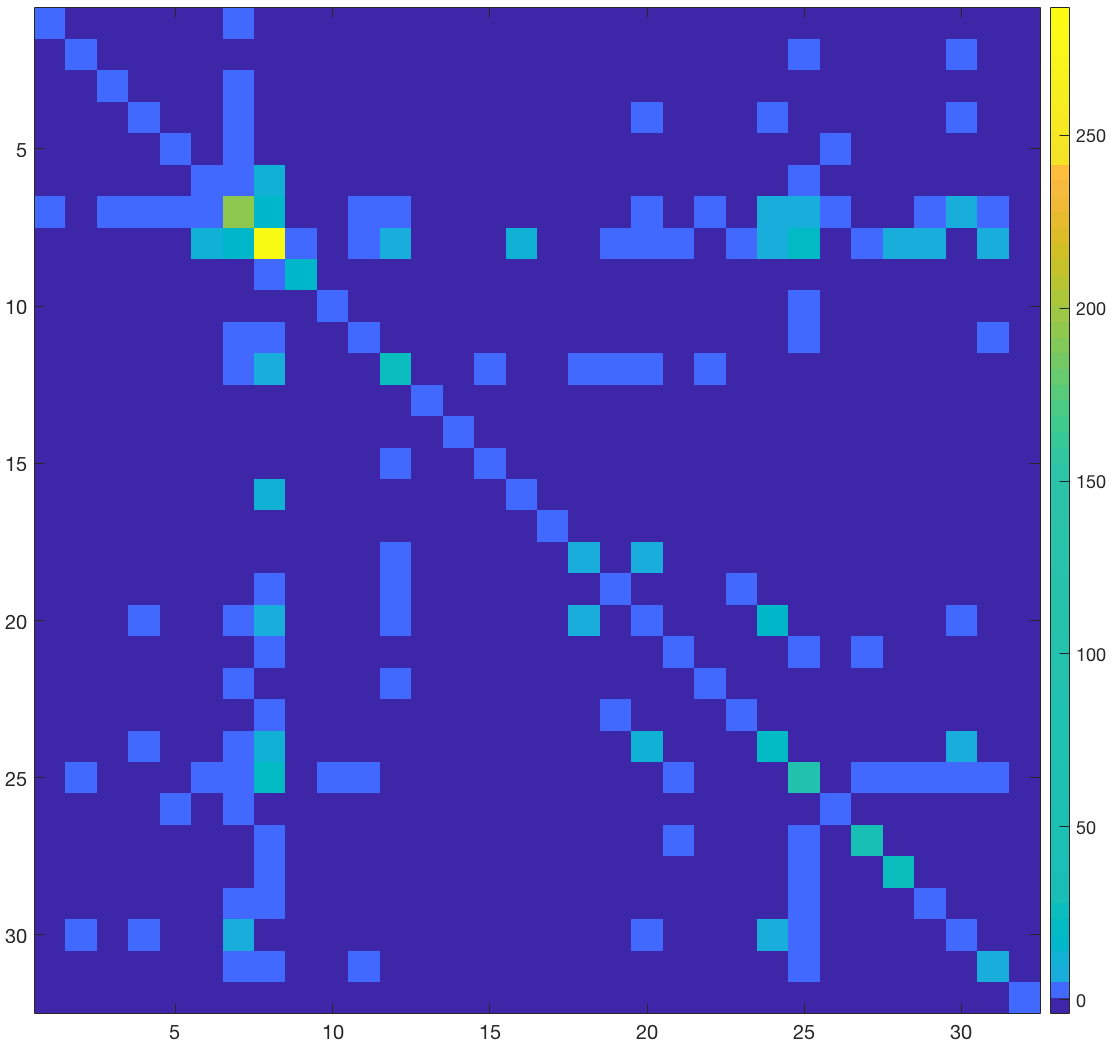
\includegraphics[height=4.5cm]{img/Analysis/image_W.png}
		\label{fig:uniAdjW}
	}
	\caption{ \subref{fig:uniAdj} is the Swiss institutions adjacency matrix, \subref{fig:uniAdjW} is the organizations weighted graph}
	\label{fig:univAdj}
\end{figure}

The sparsity of a matrix is the number of zero-valued elements divided by the total number of elements; the Swiss authors adjacency matrix has sparsity equal to $8.5 \cdot 10^{-3}$ instead the one of the world authors matrix is $2.4 \cdot 10^{-4}$ (for more on sparse matrices, see~\cite[Chapter 3]{saad}).

In Figure \ref{fig:uniAdjW} (lets call this matrix U) we can see the matrix representing the weighted collaborations between Swiss universities: as we can see in the bar at the right, blue corresponds to no collaboration and while increasing the number of collaborations the color changes to yellow.
The institutions which collaborate more in Switzerland are \'{E}cole Polytechnique F\'{e}d\'{e}rale de Lausanne and ETH Z\"{u}rich which correspond to the 7th and 8th columns/rows in the matrix. These two universities collaborate both internally in the university (see the yellow squares of $U_{7,7}$ and $U_{8,8}$ entries of the matrix U)  but also with other institutions (see the 7th and 8th columns/rows of U where we have a lot of light-blue squares): for example  ETH Z\"{u}rich has 19 collaboration with Universit\`{a} della Svizzera italiana (25th column). 
We can see that most of the light-blue squares appear in the diagonal of the matrix; it means that institutions' members usually works with authors of the same organization instead of ones from a different institution.

\textcolor{red}{Add something to say why do we apply the cuthill, come influenza i metodi numerici -- Comparare nnz(L+U) con e senza RCM. Eventualmente provare con power method.}\\
I applied the Cuthill-McKee algorithm to the two authors matrices: it permutes a sparse matrix that has a symmetric sparsity pattern into a band matrix form with a small bandwidth.
A band matrix is a sparse matrix whose non-zero elements are confined to a diagonal band; if the bandwidth of a symmetric matrix A is \textit{n}, it means that 
$$A_{ij} = 0  \:\: \text{ if } \:\: |j-i| > n$$
 This means that all the non zero elements are put as near as possible to the diagonal of the matrix, as we can see in Figure \ref{fig:CuthillMcKee}. 
 
For the matrix of Swiss authors in \ref{fig:CuthillMcKeeS} the bandwidth is 48, instead the one of the authors from all the world \ref{fig:CuthillMcKeeW} has a bandwidth of 1210. 

We can notice that in both figures the number of non-zero elements, written below the graph, doesn't change; in fact, the reverse Cuthill-McKee ordering consists only in rows and columns permutations and don't change any entry of the matrix.

\begin{figure}[tb]
	\centering
	\subfigure[]{
		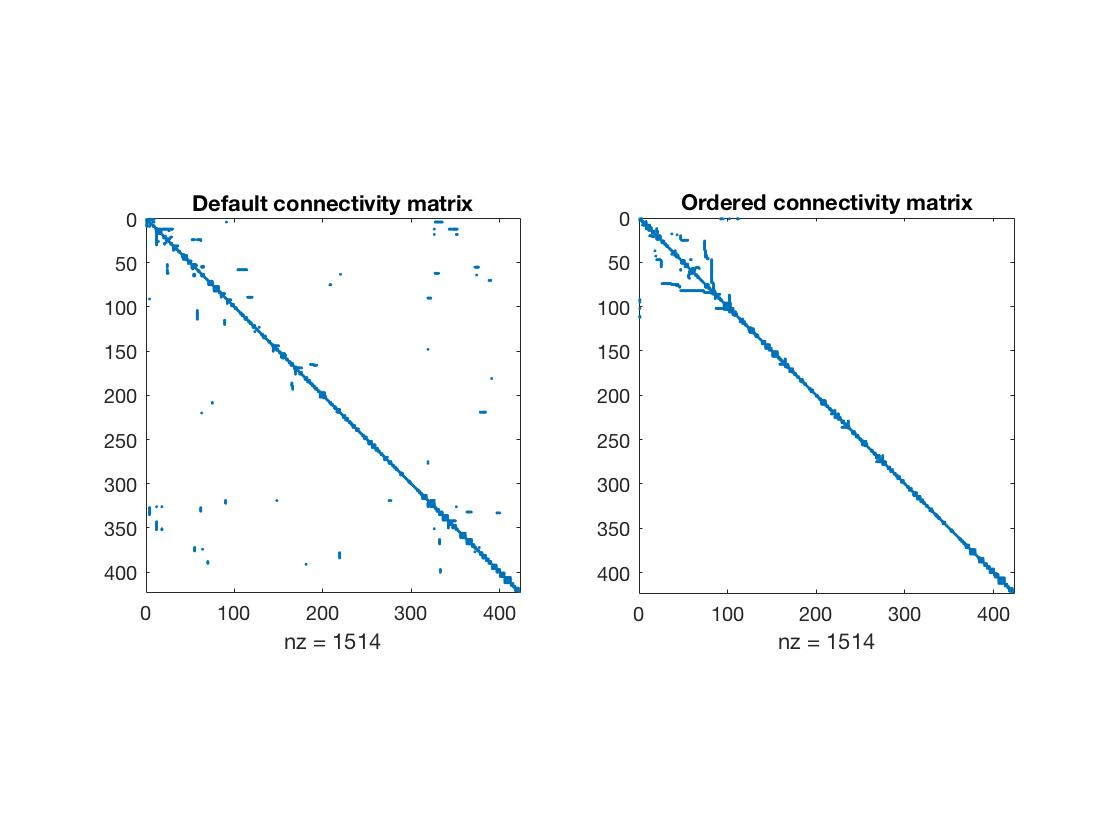
\includegraphics[height=4cm]{img/Analysis/cuthill_mckee.jpg}
		\label{fig:CuthillMcKeeS}
	}
	\subfigure[]{
		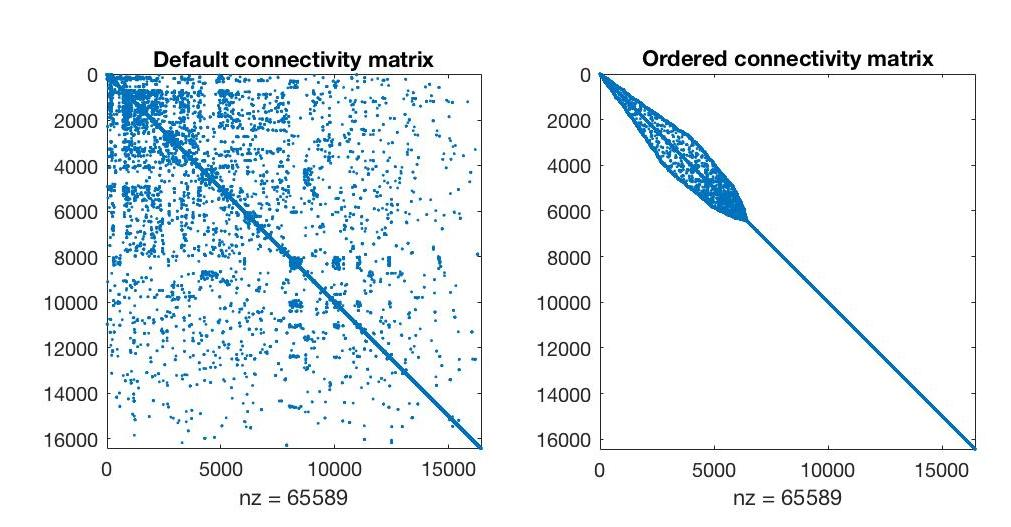
\includegraphics[height=4cm]{img/Analysis_world/cuthill_mckee.jpg}
		\label{fig:CuthillMcKeeW}
	}
	\caption{ The Reverse Cuthill McKee ordering for only Switzerland in \subref{fig:CuthillMcKeeS} and for the authors of all the world in \subref{fig:CuthillMcKeeW}}
	\label{fig:CuthillMcKee}
\end{figure}



\subsection{PageRank}
Applying the PageRank algorithm I obtain a sorted list of authors and in Figure \ref{fig:pagerank_bars} we can see all the 422 Swiss authors with their corresponding PageRank value. 

\begin{figure}[tb]
	\centering
	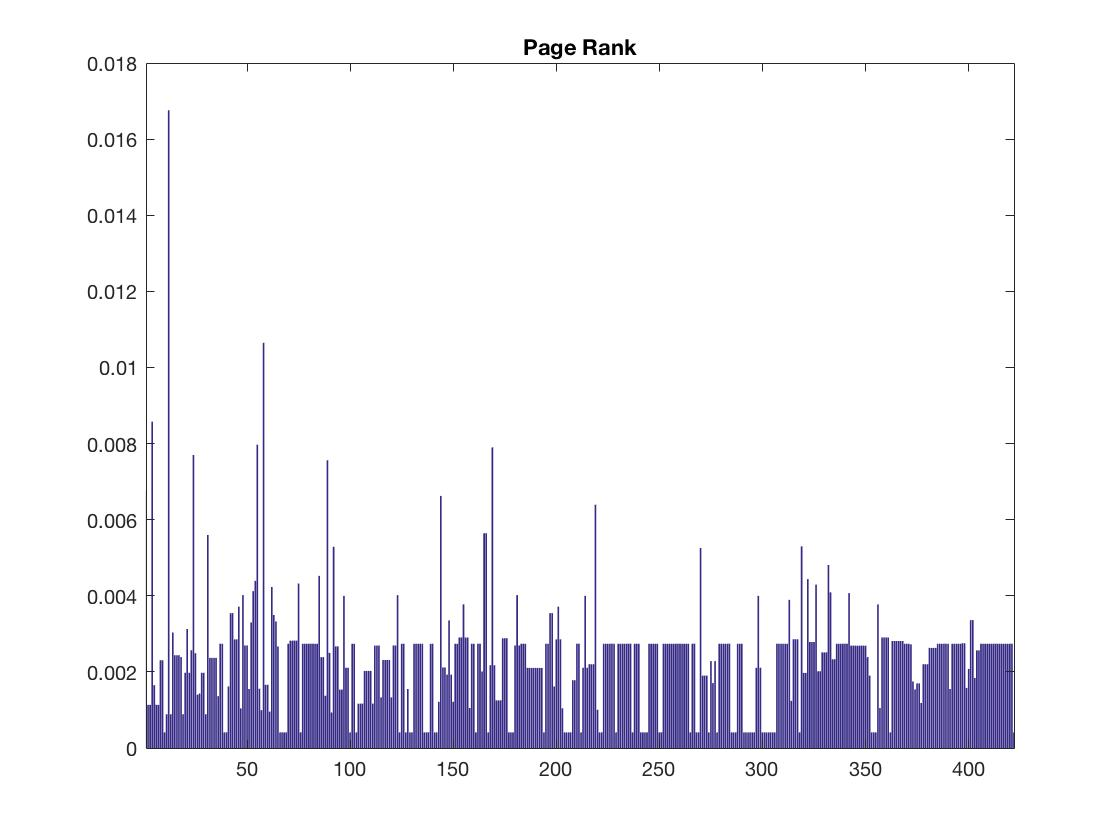
\includegraphics[height=6cm]{img/Analysis/page_rank_bars.jpg}
	\caption{ Bar graph of Swiss authors PageRank values}
	\label{fig:pagerank_bars}
\end{figure}

Table~\ref{table:PRDC}~(left) shows the first 10 most ``popular" authors sorted by the algorithm.
We can see that the \textit{In\_degree} column, which corresponds to the number of collaboration, it is not sorted because PageRank takes into account also the quality of the collaborations.
For example, the third author \textit{Simone Deparis} has more collaborations than the second \textit{Christoph Schwab}.
To see it better we can compare this table with the one on the right, containing the first 10 authors sorted only by degree-centrality (i.e., number of collaborations). The most collaborative author is still \textit{Rolf Krause} because it has 30 associations but from the second we can already see some differences in the ranking.

\newcommand\ccc{\centering}
\begin{table}[tbh]
\centering
\scriptsize
\caption{First 10 Swiss authors ranked by PageRank (left) and degree centrality (right)}
\begin{tabular}{c c m{10mm} l l}
\textbf{Index} & \textbf{PageRank} & \textbf{Degree \newline Centrality} & \textbf{Name} & \textbf{Institution}\\
\hline
12 & 0.016757 	& \ccc 30 	& Rolf Krause & USI \\
58 & 0.010648 	& \ccc 12 	& Christoph Schwab & ETHZ \\
4 & 0.0085765 	& \ccc 14 	& Simone Deparis & EPFL \\
55 & 0.0079721 	& \ccc 12 	& Costas Bekas & IBM \\
169 & 0.0078995 & \ccc 8 	& Bruno Sudret & ETHZ \\
24 & 0.0076977 	& \ccc 12 	& Peter Arbenz & ETHZ \\
89 & 0.0075607 	& \ccc 7 	& Fabio Nobile & EPFL \\
1 & 0.0067923 	& \ccc 8 	& Alfio Quarteroni & EPFL \\
144 & 0.0066262 & \ccc 7 	& Olaf Schenk & USI \\
219 & 0.0063917 & \ccc 10 	& Torsten Hoefler & ETHZ
\end{tabular}
\qquad\qquad
\begin{tabular}{c m{10mm} l}
\textbf{Index} & \textbf{Degree \newline Centrality} & \textbf{Name} \\
\hline
12 	& \ccc 30 & Rolf Krause \\
4 	& \ccc 14 & Simone Deparis \\
24 	& \ccc 12 & Peter Arbenz \\
55 	& \ccc 12 & Costas Bekas \\
58 	& \ccc 12 & Christoph Schwab \\
219 & \ccc 10 & Torsten Hoefler \\
332 & \ccc 10 & Nicolas Salamin \\
319 & \ccc 9 & Michael Afanasiev \\
1 	& \ccc 8 & Alfio Quarteroni \\
169 & \ccc 8 & Bruno Sudret
\end{tabular}
\label{table:PRDC}
\end{table}


I have also applied the PageRank algorithm to the universities adjacency matrix obtaining the results in Figure \ref{fig:PRUniversities}.
We can observe that the most present universities in the area of computational science are \'{E}cole Polytechnique F\'{e}d\'{e}rale de Lausanne, ETH Z\"{u}rich and Universit\`{a} della Svizzera italiana. Here the universities sorted by PageRank corresponds to the  sorting by number of collaborations (\textit{In\_degree} column).
\begin{figure}[tb]
	\centering
	\subfigure[]{
		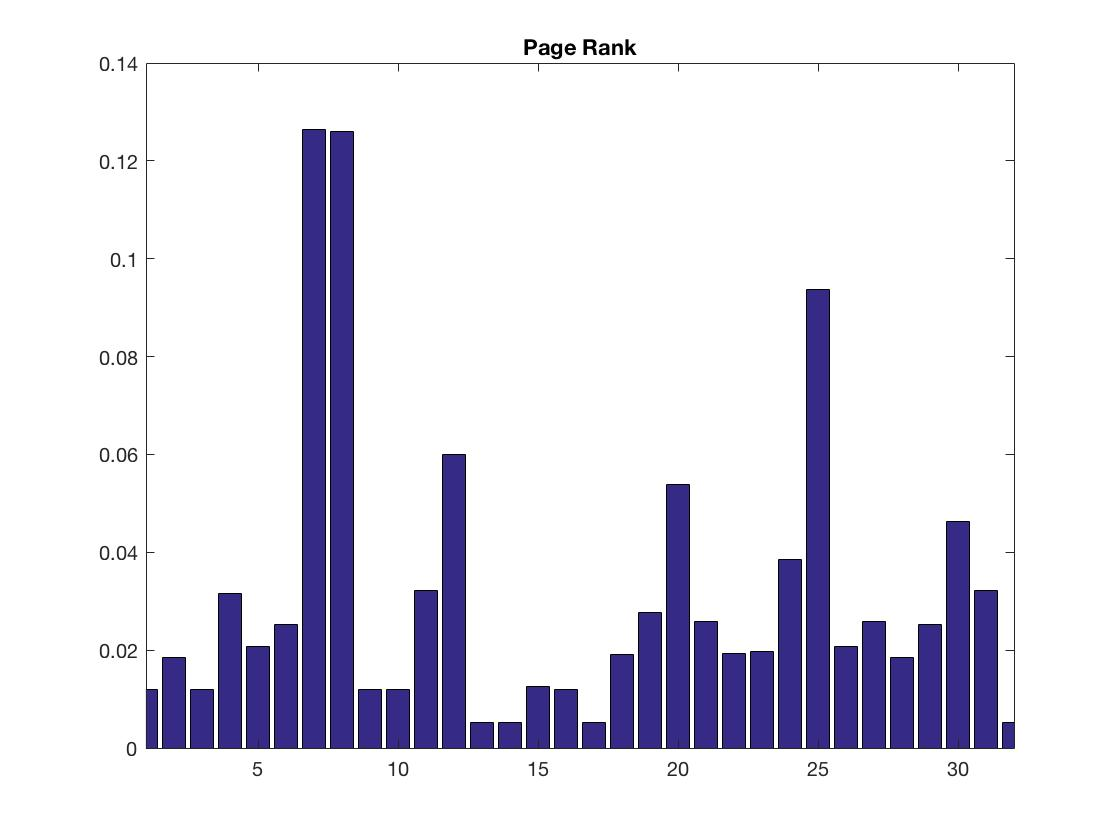
\includegraphics[height=4.5cm]{img/Analysis/page_rank_uni.jpg}
		\label{fig:PRbarsuni}
	}
	\subfigure[]{
		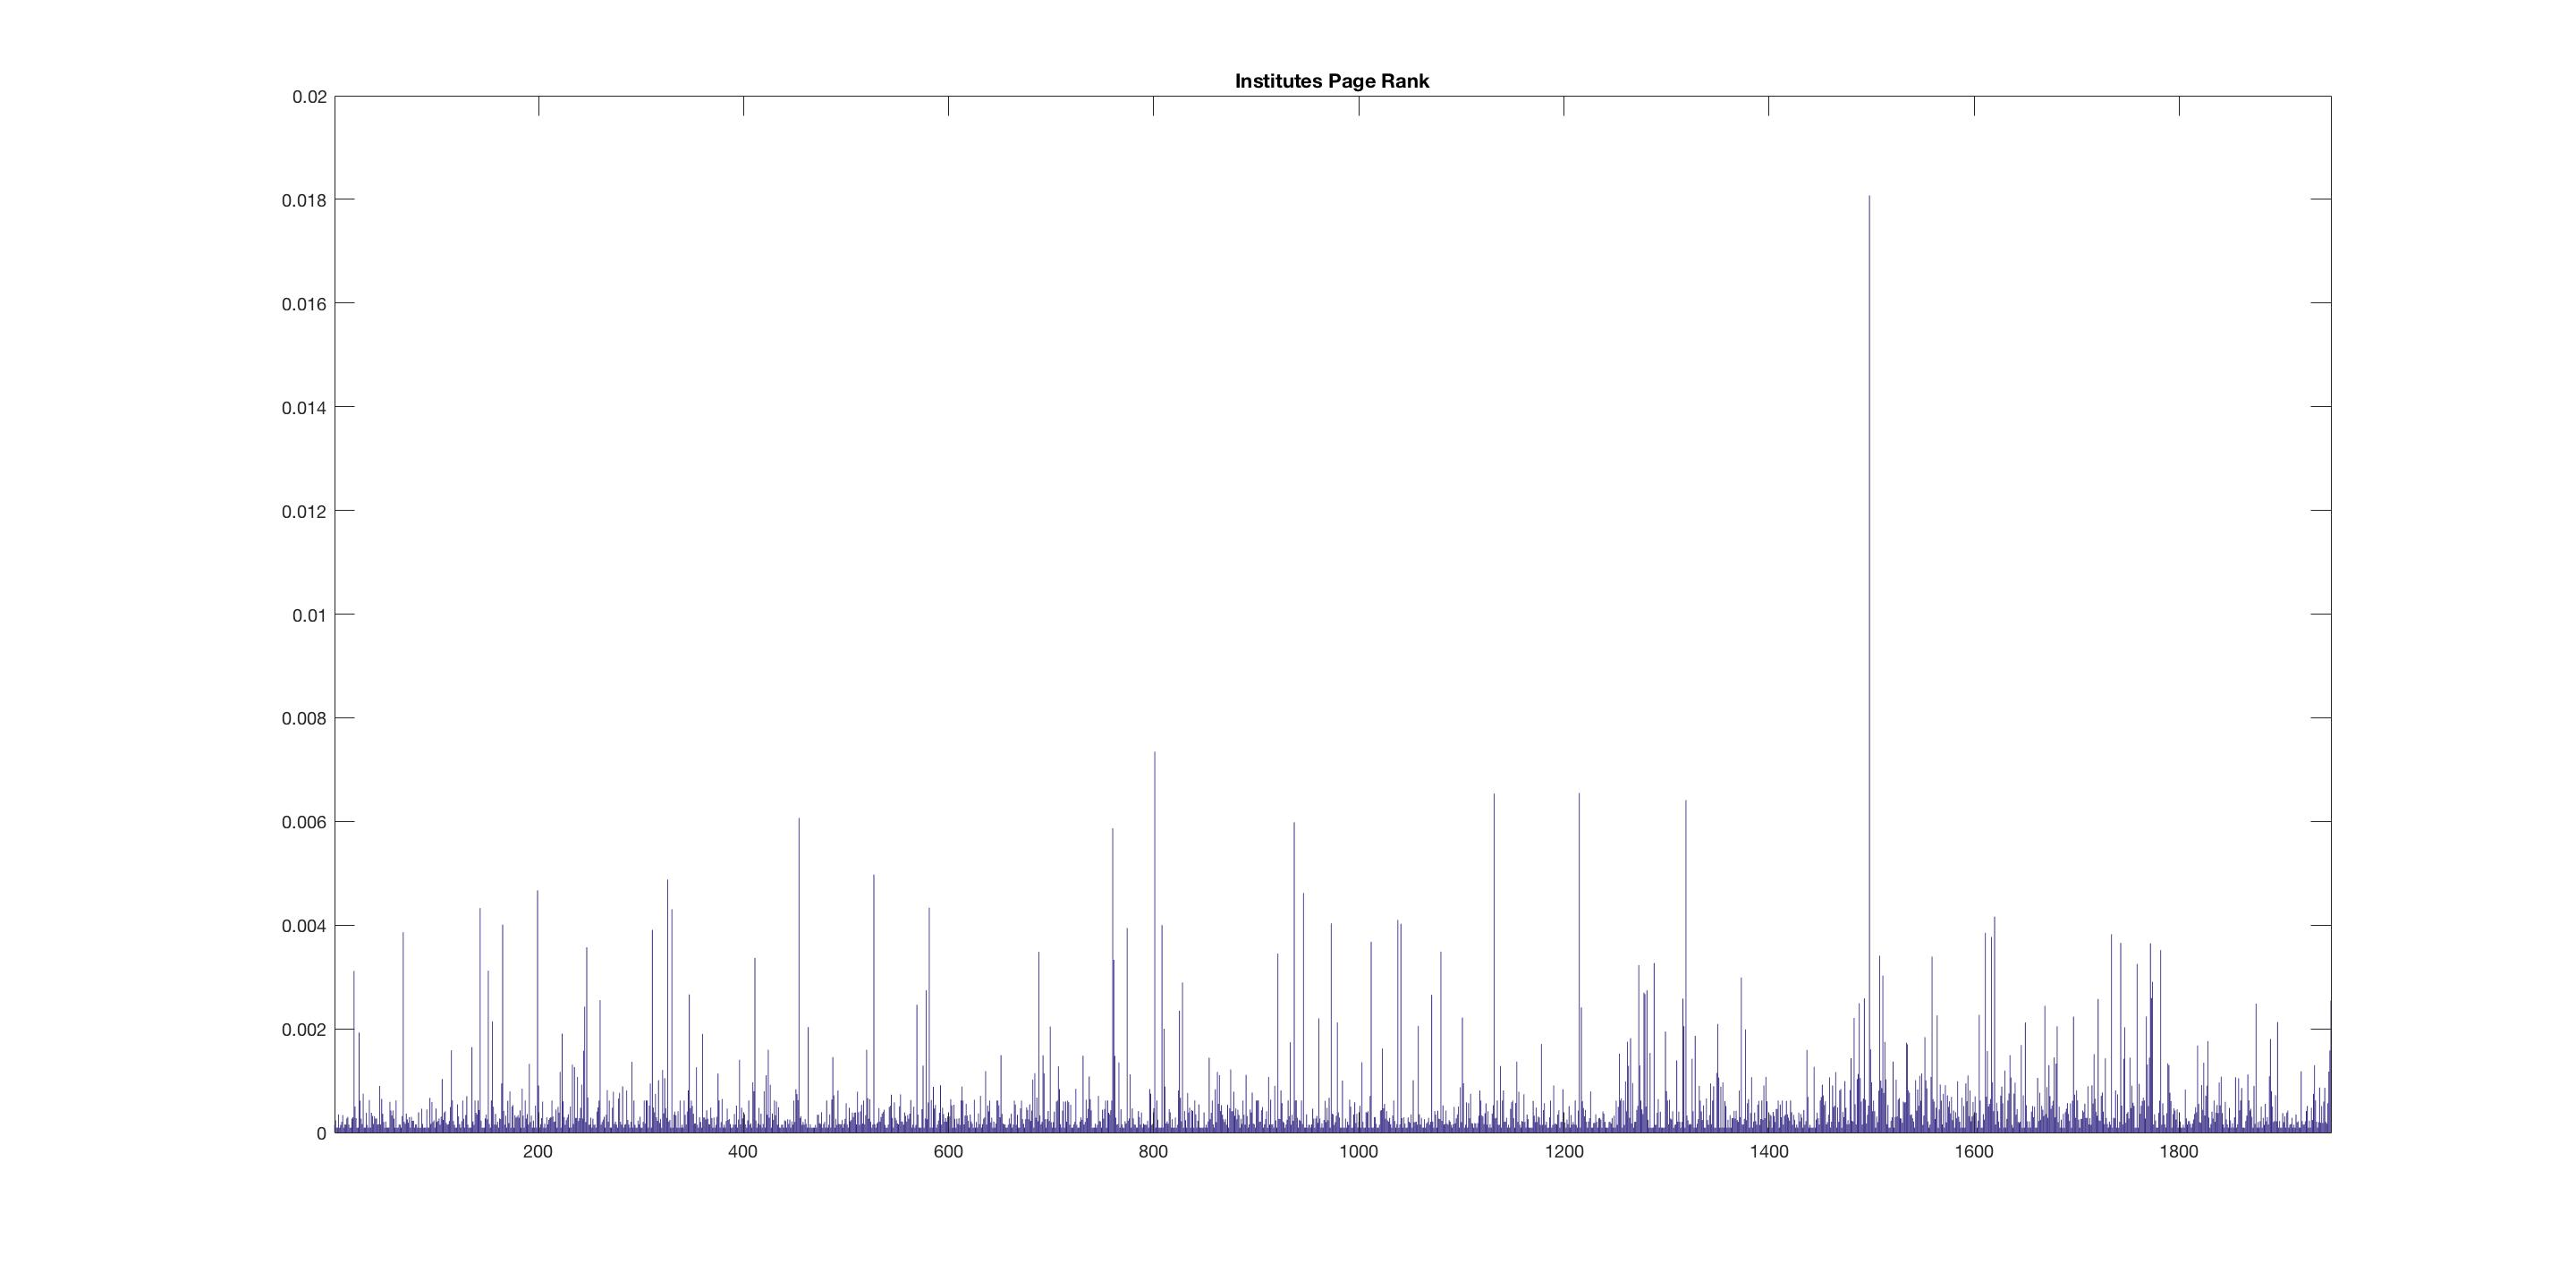
\includegraphics[height=4cm]{img/Analysis_world/pr_uni.jpg}
		\label{fig:PRlistuni}
	}
	\caption{ \subref{fig:PRbarsuni} is a bar graph of Swiss institutions PageRank values, while  \subref{fig:PRlistuni} is the one of world institutions}
	\label{fig:PRUniversities}
\end{figure}


About what concerning world information we can better see the difference between PageRank and degree centrality sorting in Table \ref{table:prW}; the Swiss  \textit{Rolf Krause}, member of USI, has the 7th PageRank value with only 38 collaborations but does not appear in the first ten positions of the degree centrality list.

\newcommand\eee{\centering}
\begin{table}[tbh]
\centering
\tiny
\caption{First 10 authors ranked by PageRank (left) and degree centrality (right)}
\begin{tabular}{c c c l l}
\textbf{Index} & \textbf{PageRank} & \textbf{D.Centrality} & \textbf{Name} & \textbf{Institution}\\
\hline
1343 & 0.00066775 & 47 & Youssef M. Marzouk & Massachusetts Institute of Technology \\
3794 & 0.00064672 & 42 & Andrea L. Bertozzi & University of California \\
2719 & 0.00055678 & 42 & Stanley J. Osher & University of California \\
115 & 0.00052919 & 49 & Omar Ghattas & The University of Texas at Austin \\
2478 & 0.00052283 & 23 & Stefan Ulbrich & Technical University Darmstadt \\
2333 & 0.0005056 & 33 & Gianluca Iaccarino & Stanford University \\
25 & 0.00049204 & 38 & Rolf Krause & USI \\
758 & 0.00047899 & 52 & Xiaoye Sherry Li & Lawrence Berkeley National Laboratory \\
701 & 0.00047145 & 51 & Eric Phipps & Sandia National Laboratories \\
773 & 0.00045236 & 41 & James W. Demmel& University of California
\end{tabular}
\qquad\qquad
\begin{tabular}{c c l}
\textbf{Index} & \textbf{Degree Centrality} & \textbf{Name} \\
\hline
715& 52 & Mark S. Shephard \\
758 & 52 & Xiaoye Sherry Li \\
701 & 51 & Eric Phipps\\
115 &49 & Omar Ghattas \\
1343 & 47 & Youssef M. Marzouk\\
188 & 44 & Siva Rajamanickam\\
189 & 43 & Erik G. Boman\\
957 & 43 & Lois Curfman McInnes\\
784 & 42 & Emmanuel Agullo \\
2719 & 42 & Stanley J. Osher
\end{tabular}
\label{table:prW}
\end{table}

Table \ref{table:PRUNI} shows the first 10 universities with higher PageRank value, the Swiss ones on the left and world information on the right: in the computational science area the most important are the University of California and the Massachusetts Institute of Technology. At ranking 10th we can find the Swiss institution, \'{E}cole Polytechnique F\'{e}d\'{e}rale de Lausanne, which was in the first position in the Swiss list.

\newcommand\ddd{\centering}
\begin{table}[tbh]
\centering
\tiny
\caption{First 10 Swiss institutions (left) and world institutions (right)  ranked by PageRank}
\begin{tabular}{c c c l l}
\textbf{Index} & \textbf{PageRank} & \textbf{D.Centrality} & \textbf{Institution}\\
\hline
7 & 0.12632 & 16 & EPFL \\
8 & 0.12601 & 16 & ETHZ \\
25 & 0.09368 & 12 & USI \\
12 & 0.059924 & 7 & IBM \\
20 & 0.053813 & 7 & SIB \\
30 & 0.046199 & 6 & University of Geneva \\
24 & 0.038438 & 5 & UNIL \\
11 & 0.032109 & 4 & HES-SO Valais-Wallais\\
31 & 0.032109 & 4 & University of Neuchatel \\
4 & 0.031569 & 4 & CHUV
\end{tabular}
\qquad\qquad
\begin{tabular}{c c c l l}
\textbf{Index} & \textbf{PageRank} & \textbf{D.Centrality} & \textbf{Institution}\\
\hline
1498 & 0.018077 & 256 & University of California \\
801 & 0.0073476 & 114 & Massachusetts Institute of Technology \\
1215 & 0.0065502 & 101 & Stanford University \\
1132 & 0.0065372 & 103 & Sandia National Laboratories \\
1319 & 0.0064138 & 97 & The University of Texas at Austin \\
454 & 0.0060685 & 92 & Georgia Institute of Technology \\
937 & 0.0059833 & 96 & New York University-NYU \\
760 & 0.0058694 & 87 & Lawrence Berkeley National Laboratory\\
527 & 0.0049737 & 80 & IBM \\
326 & 0.0048789 & 69 & EPFL
\end{tabular}
\label{table:PRUNI}
\end{table}


\subsection{Graph partitioning}
Applying the graph partitioning algorithm, the expected result was to obtain groups divided according to institution: members of the same organization will be in the same partition. This is based on the fact the the members mainly work with people of the same institution. 

I decide to apply 4-way partitioning, obtaining four groups of about 105 members.

Unfortunately the result was not what I expected because the main universities, such as \'{E}cole Polytechnique F\'{e}d\'{e}rale de Lausanne and ETH Z\"{u}rich, collaborate with almost all other institutions and for this reason appear in all the groups obtained.  

Despite all, the members of the University of Basel are almost all in the second group and the ones from USI are in the third partition.








%%%%%%%%%%%%%%%%%%%%%%%%%
\section{Conclusions} \label{sec:conclusions}
%%%%%%%%%%%%%%%%%%%%%%%%%
I have implemented some numerical methods to analyze data. The PageRank algorithm was useful to obtain 
%I have implemented an algorithm for extracting a resolution-independent vector representation from pixel art images. This algorithm resolves separation/connectedness ambiguities in the square pixel lattice and then reshapes the pixel cells so that both cardinal and diagonal neighbors of a pixel are connected through edges. The regions with smoothly varying shading are extracted and separated through piecewise smooth contour curves. I have demonstrated that conventional image upsampling and vectorization algorithms cannot handle pixel art images well, while this algorithm produces good results on a wide variety of inputs.

%\subsection{Acknowledgments}
%
%I want to thank my project advisor, prof. Kai Hormann, for suggesting this fascinating project. I really enjoyed working on it and prof. Hormann has been very helpful throughout the whole project. I was given a lot of freedom and independence, which pushed me to give the best of myself. The project had such a great potential and was so intellectually challenging that I was thrilled and eager every time I could spend time working on it.\\
%I also want to thank my wife for being so supportive and patient. The long nights passed working on this project really proved her love, and her caring for my well-being helped me a lot through the difficult and stressing moments. Her excitement for every new feature pushed me to improve the project more and more, seeking that wonderful smile.


\newpage
\bibliographystyle{plain}
\bibliography{references}

\end{document}